\begin{figure}[t]
\centering
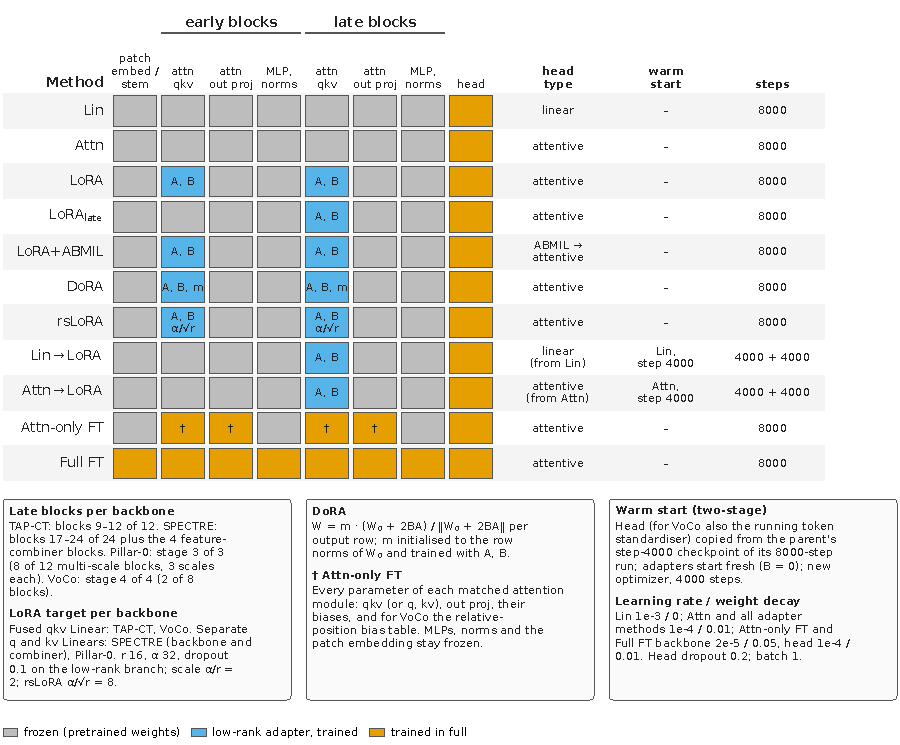
\includegraphics[width=\textwidth]{figures/fig_methods_cls.pdf}
\caption{Overview of the classification methods, drawn from the implementation: what each method trains inside every encoder block and the head (grey = frozen, blue = low-rank adapter, orange = trained in full), the head it uses, its warm start and its budget, with the late blocks and adapted projections per backbone. The data path of every backbone is drawn in Figure~\ref{fig:pipeline_cls} and the segmentation methods in Figure~\ref{fig:methods_seg} (Appendix~\ref{app:details}).}
\label{fig:methods_cls}
\end{figure}

\paragraph{Backbones.} We adapt four publicly released pretrained 3-D CT encoders of three architectural families (Figure~\ref{fig:pipeline_cls} in Appendix~\ref{app:details}). \textbf{TAP-CT-B-3D} \citep{veenboer2025tapct}, pretrained by DINOv2-style self-supervision, is a plain 12-block ViT-B \citep{dosovitskiy2021vit} with $4\times8\times8$ voxel patches, a class (CLS) token and four register tokens \citep{darcet2024registers}, applied to windows of $12\times224\times224$ voxels at native slice spacing. \textbf{SPECTRE-Large} \citep{claessens2025spectre}, pretrained by self-distillation and vision--language alignment with radiology reports, is a plain 24-block ViT-L with $16\times16\times8$ patches on crops of $128\times128\times64$ voxels at $0.5\times0.5\times1$\,mm, followed by a pretrained four-block feature combiner that attends over the crops of a volume. \textbf{Pillar-0} \citep{agrawal2025pillar0}, pretrained on CT and breast MRI of one academic centre, is used through its released head-CT encoder, a convolutional stem followed by three stages of multi-scale window-attention blocks that encode a whole $128\times256\times256$ volume from eleven intensity windows in one pass; its pretraining on head CT restricts it to the hemorrhage cohort. \textbf{VoCo-L} \citep{wu2024voco,wu2024vocolarge} is the encoder of a SwinUNETR-v2 \citep{hatamizadeh2022swinunetr,he2023swinunetrv2}, a four-stage Swin transformer \citep{liu2021swin} with patch merging between stages and no class token, applied to $96^3$ windows at 1.5\,mm; we use the released self-supervised checkpoint. Volumes are reoriented, resampled and intensity-normalised as in each backbone's pretraining (Appendix~\ref{app:details}).

\paragraph{Classification heads and methods.} Every backbone exposes a set of tokens per volume: the CLS token of every window (TAP-CT), the combiner tokens of the crops (SPECTRE), the multi-scale tokens of the whole volume (Pillar-0), or one token per window formed by the spatial means of the outputs of stages 2--4 (VoCo, 2688-dimensional). \textbf{Lin} reads a pooled feature (the mean window token, the combiner's CLS token or Pillar-0's pooled embedding) through dropout and one linear layer. \textbf{Attn} is an attentive probe \citep{bardes2024vjepa,chen2024cae}: a learnable CLS token joins the token set, two self-attention blocks run over it, and the CLS output is read out. The \numClsMethodsN{} methods differ only in what is trained inside the encoder (Figure~\ref{fig:methods_cls}): the \emph{frozen probes} Lin and Attn; \textbf{LoRA} \citep{hu2022lora} on the query, key and value projections of every block (rank 16, $\alpha=32$, dropout 0.1) and its variants \textbf{LoRA$_{\text{late}}$} (the last third of the blocks of TAP-CT and SPECTRE, the last stage of Pillar-0 and VoCo), \textbf{LoRA+ABMIL} (tokens pooled by gated attention \citep{ilse2018abmil} before the head), \textbf{DoRA} \citep{liu2024dora} and \textbf{rsLoRA} \citep{kalajdzievski2023rslora} (update scaled by $\alpha/\sqrt{r}$, four times the LoRA scale); the \emph{two-stage schedules} \textbf{Lin$\to$LoRA} and \textbf{Attn$\to$LoRA}, which train the probe for half the budget and warm-start late-block LoRA from it, in the spirit of probing before fine-tuning \citep{kumar2022lpft}; and \textbf{Attn-only FT}, which trains every parameter of the attention modules \citep{touvron2022three}, and \textbf{Full FT}, which trains every parameter. All adapted and fine-tuned models use the attentive head; Lin$\to$LoRA keeps the linear head of its parent.

\paragraph{Segmentation heads and methods.} The encoder yields a grid of tokens per crop from four depths: TAP-CT blocks 3, 6, 9 and 12 (one token per $4\times8\times8$ voxels), SPECTRE blocks 6, 12, 18 and 24 (per $8\times16\times16$ voxels) and the outputs of VoCo's four stages (strides 4 to 32). \textbf{Lin} is a $1\times1\times1$ convolution on the deepest grid, upsampled trilinearly. \textbf{Dec} is a light multi-depth decoder in the spirit of UNETR \citep{hatamizadeh2022unetr}: the four grids are projected, concatenated, fused by a $3^3$ convolution and upsampled to the voxel grid in stages (about 2.5\,M parameters, no skip connections from the input; Figure~\ref{fig:pipeline_seg}). \textbf{LoRA}, \textbf{LoRA$_{\text{late}}$} and \textbf{DoRA} add the adapters of classification under the Dec head, \textbf{Full FT} trains the encoder with it, and \textbf{Dec$\to$LoRA} trains Dec for half the budget and warm-starts all-block LoRA from it (Figure~\ref{fig:methods_seg}). Predictions are independent sigmoids per structure.

\paragraph{Per-task and joint training.} Every cohort and dataset is trained in two modes with the same data and selection rule (Figure~\ref{fig:modes}): \emph{per-task}, one model per label or structure, and \emph{joint}, one shared model with one output per label or structure. A \emph{label--mode pair} denotes one label (or structure) on one backbone in one mode. The joint classification loss sums over the labels known for a case, so a label weighs the same in both modes; the joint segmentation loss averages Dice and cross-entropy over structures. A joint model trains for the budget of one per-task model, so it uses $1/K$ of the steps of the $K$ per-task models it replaces, except where stated below.
